\section{Vergleichen von Mengen}

\begin{frame}{Vergleichen von Mengen - Jaccard-Koeffizient}
    \begin{columns} % align columns
        \begin{column}{.60\textwidth}
            \begin{itemize}
                \item Maß zum Vergleichen von zwei Mengen \pause
                \item Je näher der Jaccard-Koefficient gegen 1 geht, desto ähnlicher sind sich die Mengen \pause
                \item $ J(A,B) = \frac{ | A \cap B | }{ | A \cup B | } $ \pause
                \item Vorheriges Beispiel: $ J(S_3(A),S_3(B)) = \frac{3}{7} \approx 0.43 $ \pause
                \item Problem: $ O(n^2) $ \pause
            \end{itemize}
        \end{column}
        \hfill
        \begin{column}{.40\textwidth}
            \begin{figure}[H]
                \centering
                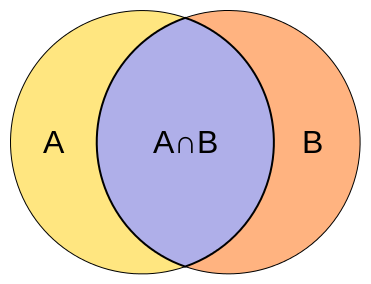
\includegraphics[width=0.75\textwidth]{images/Intersection_of_sets_A_and_B.png} 
                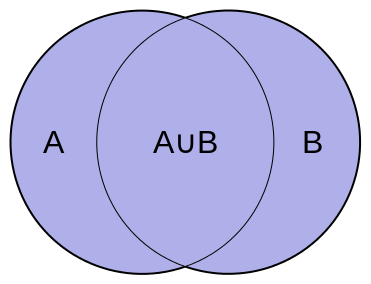
\includegraphics[width=0.75\textwidth]{images/Union_of_sets_A_and_B.png}
                \caption{Schnitt und Vereinigung zweier Mengen $ A $ und $ B $ \cite{intersectionImage,unionImage}}
            \end{figure}        
        \end{column}
    \end{columns}
\end{frame}


